\section{Forecasting wheat yields}
\label{sec:forecasting}

The econometric question asks whether heat is associated with yields. A separate, practical question is whether the weather known before harvest helps to predict them. This section answers it with a strictly chronological protocol. The answer is no, at least not better than the simplest benchmark.

\subsection{Protocol}

The protocol was fixed in a specification written before any forecast was computed (\cref{tab:specs}).
\begin{itemize}
  \item \textbf{Target and sample.} The log yield of soft wheat in the 83 departments of the main sample.
  \item \textbf{Forecast dates.} 1 June and 1 July of the harvest year. Only weather up to the day before is used: autumn, winter, spring, and May (on 1 June) or May--June (on 1 July). Nine variables per window give 36 variables, fixed in advance.
  \item \textbf{Validation.} Rolling origin: for each test year $t$ from 2016 to 2025, models are trained on 2010 to $t-1$, between 6 and 15 years. Department means, trends, standardisation and hyperparameters are all estimated within the training years. A variant trains from 1990 with the long wheat series.
  \item \textbf{Benchmarks.} B0 is the mean log yield of the department over the training years. B1 adds a common linear trend.
  \item \textbf{Models.} Each model predicts the residual of B1 from the weather variables: ordinary least squares on the variables of model M1, ridge regression, a random forest and gradient boosting. Their settings were fixed in advance; only the ridge penalty is tuned, by an inner leave-one-year-out loop on the training years.
  \item \textbf{Uncertainty.} The difference in mean squared error between a model and a benchmark is given with a 95\,\% interval from a block bootstrap over the 10 test years.
\end{itemize}
Tests check automatically that no variable uses information from after the forecast date. Some leakage cannot be removed: the SAA series were revised after the 2020 census, SIM is a reanalysis, the wheat mask comes from 2015--2017, and the 2025 yields are provisional. The sample itself is chosen with information later than some test years (the quality status published in 2025), so the exercise is a pseudo-real-time test, not a real-time one. Two smaller points: the degree-days of the last day before the forecast date use the next day's minimum temperature, which SIM measures until 18:00 UTC on the forecast day itself; and the inner loop that tunes the ridge penalty leaves out one training year at a time, so it uses training years later than the one left out. The first adds a few hours of weather after the forecast date; neither uses the yields of the test year.

\subsection{The benchmark that matters}

The specification compared models with B1. Under that pre-specified criterion, the random forest on 1 July formally qualifies as a gain: a skill of \RfVsBoneSkill\,\% with an interval excluding zero. But B1 turned out to be a weak benchmark: B0, the plain department mean, beats B1 in all \BzeroBeatsBone{} test years, because French wheat yields have plateaued (\cref{fig:wheat-yield}), so extending a trend hurts. I decided, after seeing these results, to add the comparison with B0, a benchmark already defined in the specification, and logged this change (\cref{app:deviations}). The results against B1 remain in the project tables.

There is a second consequence. The weather models were built, as specified, as corrections to B1, so they inherit its handicap: B1 itself is far worse than B0 (\cref{tab:forecast}). The comparison below therefore tests the models as pre-specified, not the value of weather as such. A model that corrects B0 instead of B1 was evaluated afterwards, on the same test years (\cref{subsec:forecast-v12}); it can only suggest what to test on new years.

\subsection{Results}

\begin{table}[H]
\centering
\small
\caption{Forecast skill relative to the department mean (B0), test years 2016--2025}
\label{tab:forecast}
\begin{threeparttable}
% GÉNÉRÉ par scripts/26_tables_memoire.py (phase5_synthese_vs_B0.csv)
\begin{tabular}{llrrr}
\toprule
Date & Model & \shortstack{Skill vs.\\B0 (\%)} & \shortstack{95\,\% interval of MSE\\difference ($\times 10^3$)} & \shortstack{Years better\\than B0} \\
\midrule
\multicolumn{5}{l}{\emph{Train from 2010}} \\
1 June & B1 (trend) & $-36$ & [$+1.2$, $+19.6$]$^*$ & 0/10 \\
1 June & OLS (M1 variables) & $-53$ & [$+3.4$, $+22.9$]$^*$ & 2/10 \\
1 June & Ridge & $-27$ & [$-1.4$, $+16.8$] & 5/10 \\
1 June & Random forest & $-15$ & [$-5.8$, $+15.2$] & 5/10 \\
1 June & Gradient boosting & $-24$ & [$-4.2$, $+18.0$] & 5/10 \\
1 July & B1 (trend) & $-36$ & [$+1.3$, $+19.7$]$^*$ & 0/10 \\
1 July & OLS (M1 variables) & $-72$ & [$+4.9$, $+31.9$]$^*$ & 1/10 \\
1 July & Ridge & $-59$ & [$-3.6$, $+36.0$] & 4/10 \\
1 July & Random forest & $-14$ & [$-5.7$, $+14.9$] & 5/10 \\
1 July & Gradient boosting & $-22$ & [$-3.7$, $+15.3$] & 4/10 \\
\multicolumn{5}{l}{\emph{Train from 1990}} \\
1 June & B1 (trend) & $-18$ & [$-1.1$, $+11.6$] & 4/10 \\
1 June & OLS (M1 variables) & $-17$ & [$-2.8$, $+14.0$] & 6/10 \\
1 June & Ridge & $+9$ & [$-4.3$, $+0.3$] & 7/10 \\
1 June & Random forest & $+9$ & [$-8.1$, $+3.5$] & 5/10 \\
1 June & Gradient boosting & $+7$ & [$-7.0$, $+3.6$] & 5/10 \\
1 July & B1 (trend) & $-18$ & [$-1.2$, $+11.4$] & 4/10 \\
1 July & OLS (M1 variables) & $-21$ & [$-0.8$, $+13.9$] & 3/10 \\
1 July & Ridge & $+20$ & [$-16.0$, $+2.4$] & 3/10 \\
1 July & Random forest & $+11$ & [$-7.8$, $+2.2$] & 5/10 \\
1 July & Gradient boosting & $+13$ & [$-6.5$, $+0.6$] & 7/10 \\
\bottomrule
\end{tabular}

\begin{tablenotes}\footnotesize
\item Skill $= 1 - \mathrm{MSE}/\mathrm{MSE}(\mathrm{B0})$, on log yield, weighted by area. Interval: 95\,\% block bootstrap over test years; $^*$: excludes zero. Positive values in the interval mean worse than B0.
\end{tablenotes}
\end{threeparttable}
\end{table}

\Cref{tab:forecast} gives the answer.
\begin{itemize}
  \item \textbf{Training from 2010:} every model does worse than B0 on average, by \ForecastBestPct\,\% to \ForecastWorstPct\,\%, and the OLS model is significantly worse.
  \item \textbf{Training from 1990:} ridge, random forest and gradient boosting do better than B0 on average, but their intervals include zero over 10 test years.
\end{itemize}
No model, as pre-specified, is significantly better than the department mean.

\begin{figure}[H]
\centering
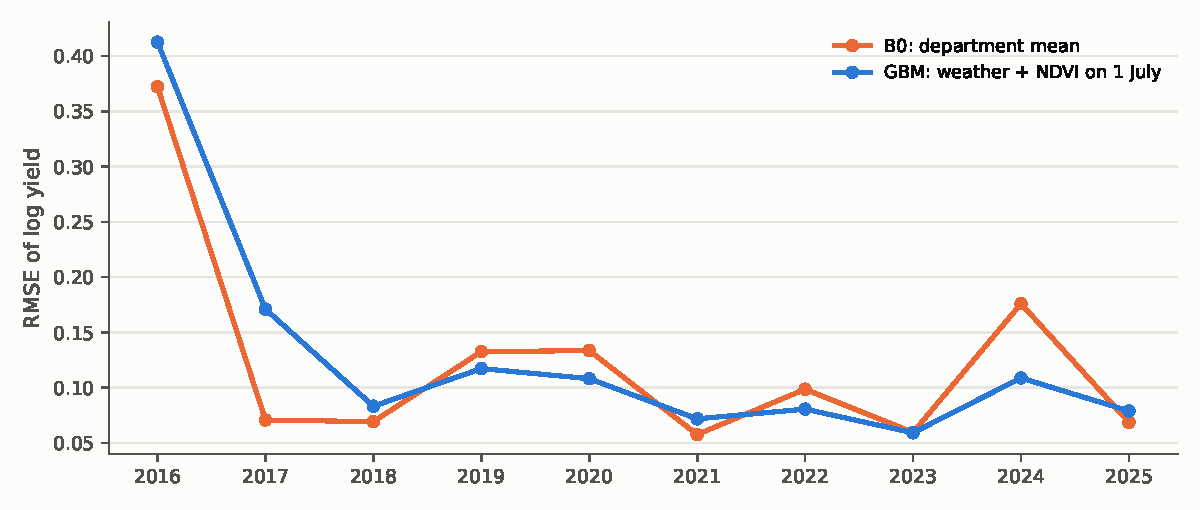
\includegraphics[width=0.95\textwidth]{figures/fig3_prevision_par_annee.pdf}
\caption{Forecast error by test year on 1 July: department mean (B0) and gradient boosting with weather and NDVI. Each model is trained only on the years before the test year.}
\label{fig:forecast-year}
\end{figure}

\subsection{Adding satellite data}

A natural objection is that weather describes the conditions, not the crop. The NDVI, a satellite index of green vegetation, describes the crop itself. I added MODIS NDVI at 250~m (16-day composites from April to June), aggregated to SIM cells and then to departments with the wheat mask. A composite is used only if it ends before the forecast date, a rule checked by an automated test.

\begin{table}[H]
\centering
\small
\caption{What NDVI adds to each model, training from 2010}
\label{tab:ndvi}
\begin{threeparttable}
% GÉNÉRÉ par scripts/26_tables_memoire.py (phase6_ndvi_synthese.csv)
\begin{tabular}{llrrr}
\toprule
Date & Model & \shortstack{Gain from NDVI vs.\\same model (\%)} & \shortstack{95\,\% interval of MSE\\difference ($\times 10^3$)} & \shortstack{Skill vs.\\B0 (\%)} \\
\midrule
1 June & Ridge & $+1.6$ & [$-1.55$, $+0.64$] & $-25$ \\
1 June & Random forest & $+1.6$ & [$-0.85$, $-0.11$]$^*$ & $-13$ \\
1 June & Gradient boosting & $+3.5$ & [$-2.26$, $-0.02$]$^*$ & $-20$ \\
1 July & Ridge & $+27.7$ & [$-22.44$, $-1.08$]$^*$ & $-15$ \\
1 July & Random forest & $+1.6$ & [$-0.95$, $+0.01$] & $-13$ \\
1 July & Gradient boosting & $+7.6$ & [$-4.55$, $-0.26$]$^*$ & $-12$ \\
\bottomrule
\end{tabular}

\begin{tablenotes}\footnotesize
\item Gain: $1 - \mathrm{MSE}(\text{with NDVI})/\mathrm{MSE}(\text{without})$. Interval of the MSE difference with minus without; $^*$: excludes zero (here, always better with NDVI).
\end{tablenotes}
\end{threeparttable}
\end{table}

NDVI helps each model a little: the gain over the same model without NDVI is positive in all \NdviTot{} cases, from \NdviGainMin{} to \NdviGainMax\,\%, and significant in \NdviSig. The largest gain, for ridge on 1 July, mostly reflects the stabilisation of a model that was unstable without NDVI. But no model with NDVI does better than the department mean, even on average (\cref{tab:ndvi}, last column). The NDVI is measured on 8~km cells weighted by wheat, not on wheat parcels alone, so it mixes crops; a parcel-level index might do better.

\subsection{What the forecasting results mean}

With 6 to 15 training years, the models as pre-specified are not significantly better than a well-chosen naive benchmark, and NDVI adds a small measurable improvement to each of them without changing that conclusion. This is consistent with earlier warnings that validation on future years is much harder than cross-validation \parencite{gouache2015,morales2023}. The main methodological point is the benchmark: had I kept the pre-specified comparison with B1 alone, I would have reported a forecasting gain over B1 that is not a gain over the simplest forecast. Whether weather can improve on B0 itself remains open.

\subsection{Correcting the department mean, and prediction intervals}
\label{subsec:forecast-v12}

The previous section left open whether weather can improve on B0. Two analyses added later, each declared in the log before it was computed, address it; both use test years that had already been seen, so they are exploratory. First, tree models built as corrections to B0 instead of B1, with the same 36 variables and the same settings, do better than B0 by \BzeroTreeMin{} to \BzeroTreeMax\,\% in mean squared error, with a 95\,\% interval that excludes zero in \BzeroTreeSig{} of the 4 cases (random forest on both dates, gradient boosting on 1 July); ridge regression does worse. This is the most promising forecasting result of the project, but it was found after B1 had been seen to fail on the same years, and it needs confirmation on the harvests from 2026, with this protocol frozen. Second, split conformal intervals \parencite{lei2018}, recalibrated each year on the residuals of earlier test years, cover \ConfCovMin{} to \ConfCovMax\,\% of departments for a nominal 90\,\%, so they are too wide: the quantile is dominated by the 2016 loss, and with so few years the intervals are not calibrated.
